\section{The pre-existing project}

The census page that contains the data in digital form holds a wealth of information about each person surveyed: name, gender, membership status and some secondary features such as work or the breed. 

All these data are housed in a moulded grid composed of numbered rows and columns. In addition to the citizens data, each archive also contains additional information related to the censor or data relating to samples of the population.

The project's objective was finding a particular grid area, corresponding to the area containing the registered State of each person, from which extract the handwritten text.

Following the words localization, the existing work proceeds by grouping visually similar elements to form a collection of homogeneous samples, in hope that each set will then contain cut outs of the same State.

The goal of the work is not to group all the words corresponding to the same state in a single cluster but rather to generate clusters that contain words that belong to a single state, the major requirement of the work is thus precision in the retrieval steps.

\subsection{Process steps}

We can summarize the project in three basic steps:
\begin{enumerate}
\item Localization of the text area containing the words of interest
\item Row segmentation
\item Post-processing and clustering
\end{enumerate}

The last step, corresponding to the feature extraction and clustering of images, is the point of interest of our paper: while the past work was focused on the localization and retrieval of the samples, not much thought was put on the features to be extracted preferring simplicity and efficiency to effectiveness.
It is this very point that gives our paper a reason d'etre: starting from the preceding, already implemented, two steps, we proceed by providing a rewritten and improved clustering method through the use of new features, these steps will be discussed later in the Section 3 and 4.

\subsubsection{Localization of the area of interest}

In this first phase the aim is to identify the region of the grid within which the State words are located. 

First of all the black border of the document is removed, an artefact resulting from the physical scanning. Then, through a vertical projection of the pixels and the creation of an histogram, the grid columns are located and, knowing the correct column's offset regarding the beginning of the document, just the one concerned is extracted.

\subsubsection{Row segmentation}

After the extraction of the concerned column from the document, we proceed with row segmentation.

Similar to the previous step, but using an horizontal projection this time, we are able to determine with some accuracy the rows of the grid. In this case, however, it's necessary to centre the word in the extracted image: this is done by correcting the height of each row by the analysis of black spikes on the created histogram.

At the end of this phase, ideally each word is contained in an individual image.

\subsubsection{Post-processing and clustering}
\label{oldFeatures}
In the post-processing phase the individual images extracted are reworked in order to remove any  vertical or horizontal residual lines left from an imperfect previous cut.

This operation of "deletion" consists in setting the related black pixels to the value of 255, pure white.
In case the spurious rows are intersected by the word additional steps are taken to leave the intersecting pixels to the original value. We find an example of this in Figure \ref{postProcessing}.

This allows us to extract the most significant features in the next steps of the process.
To extract the features each image is divided in windows with width of 1 pixel, on these windows are then applied the functions utilized for the extraction.

The preexisting project focus was the extraction of the words, placing less importance on the clustering and thus the features themselves, moreover the project philosophy is not to place excessive burden on the operating system, from these reasons  the features are relatively simplistic: for each window the features considered are the height of the first and last black pixels and the number of transitions of the pixels from black to white and vice versa.
The distance between images is found through the Euclidean Distance where the considered axis are the number of transitions and the stroke height calculated through a simple subtraction of the first and last black pixels height.
The distance matrix is then fed to the Affinity Propagation algorithm to create the desired clusters.

\begin{figure}[!ht]
\centering
\vspace{0.3cm}
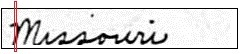
\includegraphics[width=0.5\textwidth]{images/missouri_1pix.jpg}
\caption{An image extracted from document, the red box delineates the 1 pixel wide window.}
\label{fig:extracted_image}
\end{figure}

As you can see in Figure \ref{fig:extracted_image} representing an extracted image, the word is centered and the bottom presents a white line: the bottom border row of the grid was intersecting the word and was extracted with it, in the pre-processing phase it was thus removed to not hinder the feature extraction.

\subsection{Problems}

The localization of words and their segmentation has inherent persistent difficulties.

A first error source is represented by the inherent document skew. The skew may be due to a not perfectly horizontal scan of the original document, its presence reduces the efficacy of the work in searching for rows and columns of the grid, making the segmentation impossible with the given implementation of the project.

Other source of errors is the presence in some scanned images of other census forms below the current one: black columns from the lower document are seen as belonging to the upper one, making the application recognize them as the first column of the form.


This erroneous association renders the scan unusable since the targeted state area is found from the first black column through an hard-coded distance in pixels, moreover the analysis of the scan introduces in the clustering phase incorrect images that, recognised as similar, due to the particular way the code is implemented, skew the results in favour of the application increasing the supposed precision. 

\begin{figure}[!htpb]
\centering
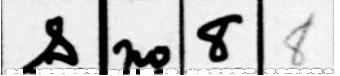
\includegraphics[width=0.26\textwidth]{images/wrongColumn.jpg}
\caption{The resulting erroneous images}
\label{err}
\end{figure} 

The identification of extraneous lines is another source of difficulties: the large number of dashed lines present makes the correct recognition extremely hard, it isn't always possible to \emph{clean} the images and this can cause errors in the clustering phase.

\begin{figure}[!htpb]
 \centering
 \subfigure[An image with a dashed line]
   {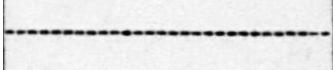
\includegraphics[width=0.3\textwidth]{images/img3.jpg}}
 \hspace{5mm}
 \subfigure[The line intersects the word]
   {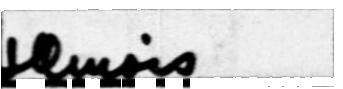
\includegraphics[width=0.3\textwidth]{images/img4.jpg}}
 \caption{Segmentation and post-processing issues}
 \label{postProcessing}
 \end{figure}
\hspace{1mm}
In other cases the word intersects directly gridlines. Because of this we may experience a loss of information about words if the line is removed using the method described above.



Regarding the previous source of errors many have been corrected in the new implementation:
through a more precise and thorough identification of the first black column the erroneous segmentation resulting in samples similar to Figure \ref{err} has been rendered not feasible; the problems stemmed from the difficult phase of cleaning the segmented images have been skirted through the removal of the steps to clean intersecting lines altogether, the presence of a black line doesn't generate problems for the new features' detection.

A problem of the old implementation is also the way the features extraction and the pre-processing are administered: while they could all be realized within the threads that extracted the words, they are instead left for later to be processed single-thread, causing unnecessary slowing downs. This is remedied in the new implementation. 